\documentclass[a4paper]{article}

\usepackage{lmodern}

%% Language and font encodings
\usepackage[french]{babel}
\usepackage[utf8x]{inputenc}
\usepackage[T1]{fontenc}
\usepackage{enumitem}
\usepackage{xcolor}
\usepackage{pifont}

%% Sets page size and margins
\usepackage[a4paper,top=3cm,bottom=3cm,left=2cm,right=2cm,marginparwidth=2cm]{geometry}
%% Useful packages
\usepackage{amsmath}
\usepackage{graphicx}
\usepackage[colorinlistoftodos]{todonotes}
\usepackage[colorlinks=true, allcolors=black]{hyperref}
\usepackage{fourier-orns}
\usepackage{titlesec}
\usepackage{fancyhdr}
\usepackage{fancyvrb}
%\renewcommand{\thefootnote}{\*}
\pagestyle{fancy} 
\setcounter{tocdepth}{5}
\usepackage{array}



%% Tikz stuff
\usepackage{tikz}
\usetikzlibrary{calc, arrows}
\tikzstyle{incolore} = [rectangle, rounded corners, draw=black, minimum height=1cm, minimum width=3cm, text width=3cm, text centered]
\usepackage{float}

\usepackage{makecell}
\usepackage{libertine}
\newcommand{\hsp}{\hspace{20pt}}
\newcommand{\HRule}{\rule{\linewidth}{0.5mm}}





\renewcommand{\headrulewidth}{1pt}
\fancyhead[C]{} 
\fancyhead[L]{}
\fancyhead[R]{\footnotesize{\leftmark}}

\renewcommand{\footrulewidth}{1pt}
\fancyfoot[C]{} 
\fancyhead[L]{}
\fancyfoot[R]{\thepage}

\definecolor{Zgris}{rgb}{0.87,0.85,0.85}

\usepackage{eso-pic,graphicx}
\usepackage{xcolor}
\newcommand{\bgimg}[1]{
\AddToShipoutPicture
   {
      \put(\LenToUnit{0 cm},\LenToUnit{0 cm})
      {
            \includegraphics[width=\paperwidth,height=\paperheight]{#1} 
      }
   }
}


\begin{document}
\begin{titlepage}
    \begin{sffamily}
        \begin{center}
            \textnormal{}\\[6.5cm]
            \HRule \\[0.4cm]
            { \Huge \bfseries Synthèse Théorique\\ Principes de cryptographie\\ Partie 1\\ [0.4cm] }
            \HRule \\[3cm]
            \Large
            Tout jusqu'à la distribution quantique des clés\\
            Deuxième Bloc\\
            Sécurité des systèmes\\
            Année académique 2020-2021\\[0.5cm]
            \emph{Rédigé par}\\
            \emph{Sénéchal Julien}
            \vfill
            {\large 21 Décembre 2020}
        \end{center}
    \end{sffamily}
\end{titlepage}

\section{Histoire}
\subsection{Scytale}
\begin{itemize}[label=\textbullet, font=\Large]
    \item Le message vient s'enrouler au tour de la Scytale
    \item Clé : l'épaisseur de la scytale
\end{itemize}

\subsection{Atbash}
\begin{itemize}[label=\textbullet, font=\Large]
    \item Chiffrement par substitution inversée
    \item Clé : Nombre de lettres et sens du décalage
\end{itemize}
\begin{figure}[H]
    \centering
    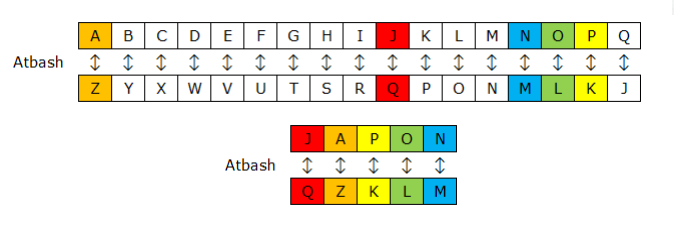
\includegraphics[width=15cm]{images/atbash.PNG}
    \caption{Atbash}
\end{figure}

\subsection{Chiffre de César}
\begin{itemize}[label=\textbullet, font=\Large]
    \item Consiste à décaler les lettres de l'alphabet d'un nombre $n$
    \item Clé : Nombre de lettres de décalage
    \item Peu sûr car peu de configuration possible (25 possibilité)
\end{itemize}

\subsection{Cryptanalyse : al-Kindi}
\begin{itemize}[label=\textbullet, font=\Large]
    \item Analayse la fréquence des lettres du texte chiffré et le compare avec la moyenne des lettres utilisé dans la langue
    \item Utile pour une substitution monoalphabétique
\end{itemize}

\subsection{Le cadran d'Alberti}
\begin{itemize}[label=\textbullet, font=\Large]
    \item Chiffrement polyalphabétique
    \item 2 cadran, l'un avec les lettres dans l'ordre et l'autre dans le désordre
    \item On aligne les 2 "A" et toutes les 4 lettres on tourne d'une lettre le petit disque
    \item Suffit de posséder le cadran pour le décrypter
\end{itemize}

\subsection{Vigenère}
\begin{itemize}[label=\textbullet, font=\Large]
    \item Intersection entre la lettre en clair et celle de la clé
    \item Simple et sûr si la clé sécurisée
    \item Analyse de fréquence inutile
    \item Substitution polyalphabétique par bloc
\end{itemize}
\begin{figure}[H]
    \centering
    
\includegraphics[width=7cm]{images/vigenere1.PNG}
    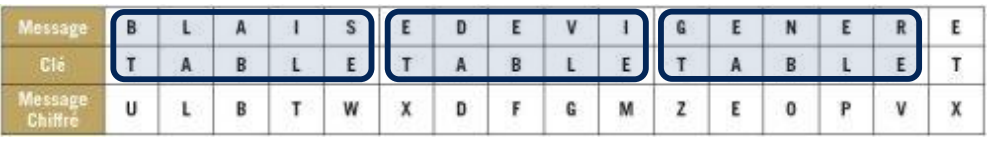
\includegraphics[width=10cm]{images/vigenere2.PNG}
    \caption{Vigenère}
\end{figure}

\subsection{Chiffre de Playfair}
\begin{itemize}[label=\textbullet, font=\Large]
    \item Chiffrement parblocs de 2 lettres
    \item Clé : Phrase du tableau de 5 x 5
    \item Très dur a casser par analyses fréquentielles
\end{itemize}
\begin{figure}[H]
    \centering
    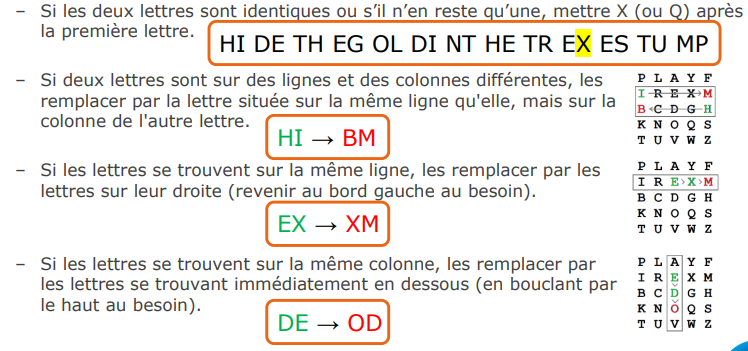
\includegraphics[width=10cm]{images/playfair.PNG}
    \caption{Playfair}
\end{figure}

\subsection{Principe de Kerckoffs}
\begin{itemize}[label=\textbullet, font=\Large]
    \item Les systèmes doivent être totalement publics
    \item Le message est sûr tant que la clé est secrète
    \item Toute attaque contre le cryptosystème doit être envisagée en considérant que l'attaquant connaît tous les détails de conception du système cible
\end{itemize}

\subsection{Chiffre de Vernam}
\begin{itemize}[label=\textbullet, font=\Large]
    \item Chiffre parfaitement sûr (que même avec le message chiffré et une puissance de calcul infinie, il est impossible de retrouver le message en clair)
    \item 3 impératifs
    \begin{itemize}[label=\ding{228}, font=\scriptsize]
        \item Aussi longue que le texte à chiffrer
        \item Parfaitement aléatoire
        \item Utilisée pour chiffrer un seul message puis est immédiatement détruite
    \end{itemize}
    \item Inconvénient
    \begin{itemize}[label=\ding{228}, font=\scriptsize]
        \item clé très longues
        \item parfaite synchro des clés
        \item échange des clés doit être sécurisé
        \item parfaitement aléatoire > très difficile
    \end{itemize}
\end{itemize}

\subsection{Enigma}
\begin{itemize}[label=\textbullet, font=\Large]
    \item Basé sur le chiffre de vigenère de longueur 26 (26 nombre de rotors)
\end{itemize}

\section{Vocabulaire}
\begin{itemize}[label=\textbullet, font=\Large]
    \item Cryptographie
    \begin{itemize}[label=\ding{228}, font=\scriptsize]
        \item Science consistant à écrire l'information pour la rendre inintelligiblle à ceux qui ne possèdent pas les capacités de la déchiffrer
    \end{itemize}
    \item Chiffrement
    \begin{itemize}[label=\ding{228}, font=\scriptsize]
        \item Opération par laquelle on chiffre le message, c’est une opération de codage
        \item Chiffrer = cryptographier ≠ crypter
    \end{itemize}
    \item Déchiffrer
    \begin{itemize}[label=\ding{228}, font=\scriptsize]
        \item Se fait avec la clé de chiffrement
    \end{itemize}
    \item Décrypter
    \begin{itemize}[label=\ding{228}, font=\scriptsize]
        \item Lorsqu'on a pas la clé
    \end{itemize}
    \item Cryptanalyse
    \begin{itemize}[label=\ding{228}, font=\scriptsize]
        \item Ensemble des moyens permettant d’analyser une information chiffrée afin de la décrypter.
    \end{itemize}
\end{itemize}

\section{Principes de base}
\begin{itemize}[label=\textbullet, font=\Large]
    \item Les algorithme publics sont plus robustes
    \item La taille de la clé est primordiale
    \item Le secret du message chiffré est basé sur le secret de la clé et non de l’algorithme
\end{itemize}

\section{Outils de base}
\begin{itemize}[label=\textbullet, font=\Large]
    \item XOR 
    \begin{itemize}[label=\ding{228}, font=\scriptsize]
        \item Méthode fondamentale
        \item Très simple
        \item Pas sécurisé
        \item Principe : Vrai si une seule des 2 entrées est vraie en binaire
    \end{itemize}
    \item Substitution
    \begin{itemize}[label=\ding{228}, font=\scriptsize]
        \item Remplacer chaque lettre du texte en clair par une autre lettre
        \item Le destinataire fait l'inverse
        \item Substitution arbitraire : Mise en place d'une table de conversion, chaque lettre remplace une autre de façon arbitraire
        \item Substitution par rotation : Code de césar avec un nombre $n$ de rotation
    \end{itemize}
    \item Hybride
    \begin{itemize}[label=\ding{228}, font=\scriptsize]
        \item Une des techniques ci-dessus $\rightarrow$ Facilement décryptable
        \item Les différents outils de chiffrement sont combinés pour obtenir un chiffrement plus robuste
    \end{itemize}
\end{itemize}

\section{Chiffrement symétrique}
\begin{itemize}[label=\textbullet, font=\Large]
    \item Base
    \begin{itemize}[label=\ding{228}, font=\scriptsize]
        \item Cryptographie a clé secrète
        \item Même clé pour le chiffrement et le déchiffrement
    \end{itemize}
    \item Longeur de la clé
    \begin{itemize}[label=\ding{228}, font=\scriptsize]
        \item L'attaque la plus simple pour récupérer la clé est l'attaque par Brute Force $\rightarrow$ Pour contrer : augmenter la taille de la clé
    \end{itemize}
    \item Echange de la clé
    \begin{itemize}[label=\ding{228}, font=\scriptsize]
        \item Il faut un canal de transmission de clé très sécurisé
    \end{itemize}
    \item Distribution des clés
    \begin{itemize}[label=\ding{228}, font=\scriptsize]
        \item Chaque couple d'interlocuteurs doit posséder sa clé secrète
        \item $n$ personnes nécessitent $\frac{n*(n-1)}{2}$ clés
    \end{itemize}
    \item Avantages
    \begin{itemize}[label=\ding{228}, font=\scriptsize]
        \item Nécessite des clés de taille relativement faible (128 bits)
        \item Consomme peu de ressources
        \item Peut chiffré en temps réel ou différé
    \end{itemize}
    \item Exemples
    \begin{itemize}[label=\ding{228}, font=\scriptsize]
        \item DES 
        \item 3DES 
        \item RC2, RC4, RC5
        \item IDEA 
        \item Blowfish 
        \item AES
    \end{itemize}
\end{itemize}

\section{Chiffrement asymétrique}
\begin{itemize}[label=\textbullet, font=\Large]
    \item Analogie
    \begin{enumerate}
        \item Alice envoie de la clé publique c'est comme si on envoyait une valise avec un cadenas ouvert
        \item Bob mets son message dans la valise et la referme avec le cadenas (donc chiffre le message avec sa clé publique)
        \item Alice ouvre la valise avec sa clé secrète qui est la clé du cadenas
    \end{enumerate}
    \item Lien entre la clé privée et la clé publique
    \begin{itemize}[label=\ding{228}, font=\scriptsize]
        \item Les 2 clés sont liées par des problèmes mathématiques extrêmement difficiles à résoudre
        \item Des fonctions trappes sont utilisées pour cela, elles ont la particularité d'être facile à calculer dans un sens mais presque impossible dans le sens inverse. 
        Le sens moyen de faire le calcul inverse est de connaître la trappe
        \item Exemple : 
        \begin{itemize}
            \item Il est facile de faire $3^5 = 243$ mais beaucoup moins simple de faire le calcul inverse qui est $log_x y = 243$ car on ne connaît pas la paire de $x y$
        \end{itemize}
        \item Les algorithmes réels utilisent des nombres premiers, ils peuvent avoir plusieurs centaines de chiffres.        
    \end{itemize}
    \item Congruence
    \begin{figure}[H]
        \centering
        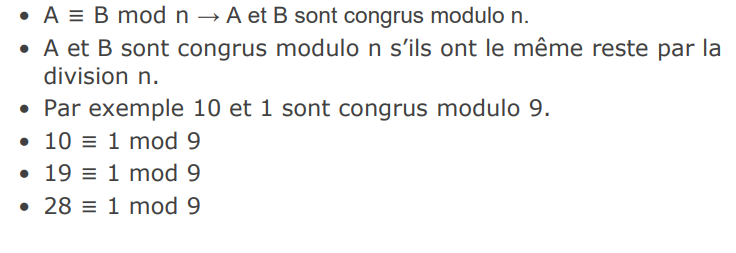
\includegraphics[width=8cm]{images/congruence.PNG}
        \caption{Congruence}
    \end{figure}
    \item Exemples :
    \begin{itemize}[label=\ding{228}, font=\scriptsize]
        \item RSA (Basé sur la factorisation en nombres premiers)
        \item Diffie-Henman (Basé sur le calcul des logarithme discret)
    \end{itemize}
\end{itemize}

\section{Fonction de hachage}
\begin{itemize}[label=\textbullet, font=\Large]
    \item Transforme la donnée initiale en une donnée numérique de taille fixée de faible longueur appellé hash
    \item Le hash est l'empreinte de la donnée initiale
    \item Généralement entre 128 et 256 bits
    \item Propriété :
    \begin{itemize}[label=\ding{228}, font=\scriptsize]
        \item La longueur de l’empreinte est toujours la même, quelle que soit la longueur du
        message en entrée.
        \item Cette empreinte doit être unique. Deux messages, même très proches ont une
        empreinte différente.
        \item La fonction de hachage doit être une fonction à sens unique afin qu’il ne soit pas
        possible, à partir de la signature, de remonter au message initial.
    \end{itemize}
    \item Concepts
    \begin{itemize}[label=\ding{228}, font=\scriptsize]
        \item Si un bit de donnée en entrée est modifié, chaque bit de sortie a
        50\% de chance de changer
        \item Le but du hash est de s'assurer de l'intégrité de la donnée
        \item Font partie des signatures numériques et sont utilisé pour stocker les mdp
    \end{itemize}
    \item Exemples :
    \begin{itemize}[label=\ding{228}, font=\scriptsize]
        \item SHA-1 SHA-256 SHA-384 SHA-512 (Secure Hash Algorithm)
        \item HAVAL
        \item RIPE-MD
        \item MD2, MD4, MD5, MD6
    \end{itemize}
\end{itemize}

\section{Signature Numérique}
\begin{itemize}[label=\textbullet, font=\Large]
    \item Principe
    \begin{itemize}[label=\ding{228}, font=\scriptsize]
        \item L'émetteur va envoyer un document et va envoyer son empreinte qui elle sera chiffrée par sa clé privée
        \item Le destinataire va alors déchiffrer l'empreinte avec la clé publique (comme il arrive a le déchiffrer, l'emprunte vient bien du bon emetteur)
        \item Le destinataire va ensuite recalculer l'emprunte du document et le comparer avec l'emprunte reçue
    \end{itemize}
\end{itemize}

\section{Clé de session}
\begin{itemize}[label=\textbullet, font=\Large]
    \item Optimisation par clé de session
    \begin{itemize}[label=\ding{228}, font=\scriptsize]
        \item Chiffrement asymétrique lent (clé d'environ 2048 bits)
        \item Chiffrement symétrique rapide mais problème de distribution des clés
        \item Solution : On combine les deux
        \begin{enumerate}
            \item Pour chiffrer un message de grande taille, on le chiffre avec une clé de session symétrique à usage unique
            \item La clé de session est chiffrée avec la clé publique du destinataire
            \item On envoie le message et la clé
            \item Le destinataire déchiffre la clé de session grâce à sa clé privée
            \item Il peut maintenant déchiffrer le message
            
        \end{enumerate}
    \end{itemize}
\end{itemize}
\begin{figure}[H]
    \centering
    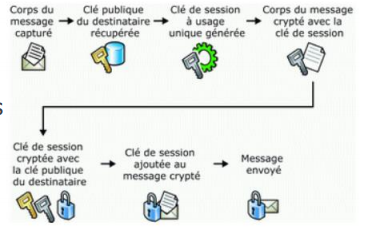
\includegraphics[width=7cm]{images/session 1.PNG}
    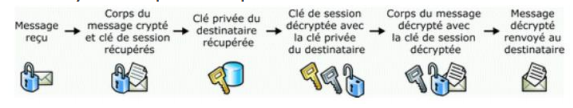
\includegraphics[width=10cm]{images/session2.PNG}
    \caption{Echange de la clé de session}
\end{figure}

\section{Signature numérique et Clé de session}
\begin{itemize}[label=\textbullet, font=\Large]
    \item L'expediteur
    \begin{enumerate}
        \item On hash le message 
        \item On chiffre la hash avec la clé privée de l'expéditeur
        \item On ajoute le hash chiffré au message et on chiffre le tout avec la clé de session
        \item On chiffre la clé de session avec la clé publique du destinataire et on l'envoie avec le pack "hash + message" chiffré
    \end{enumerate}
    \item Le destinataire
    \begin{enumerate}
        \item La clé de session est déchiffrée grâce à la clé privée du destinataire
        \item On déchiffre le pack "hash + message" avec cette clé de session
        \item On calcule le hash du message
        \item On déchiffre le hash reçu grâce à la clé publique de l'expéditeur
        \item On compare les 2 hash et si ils correspondent, tout est bon
    \end{enumerate}    
\end{itemize}
\begin{figure}[H]
    \centering
    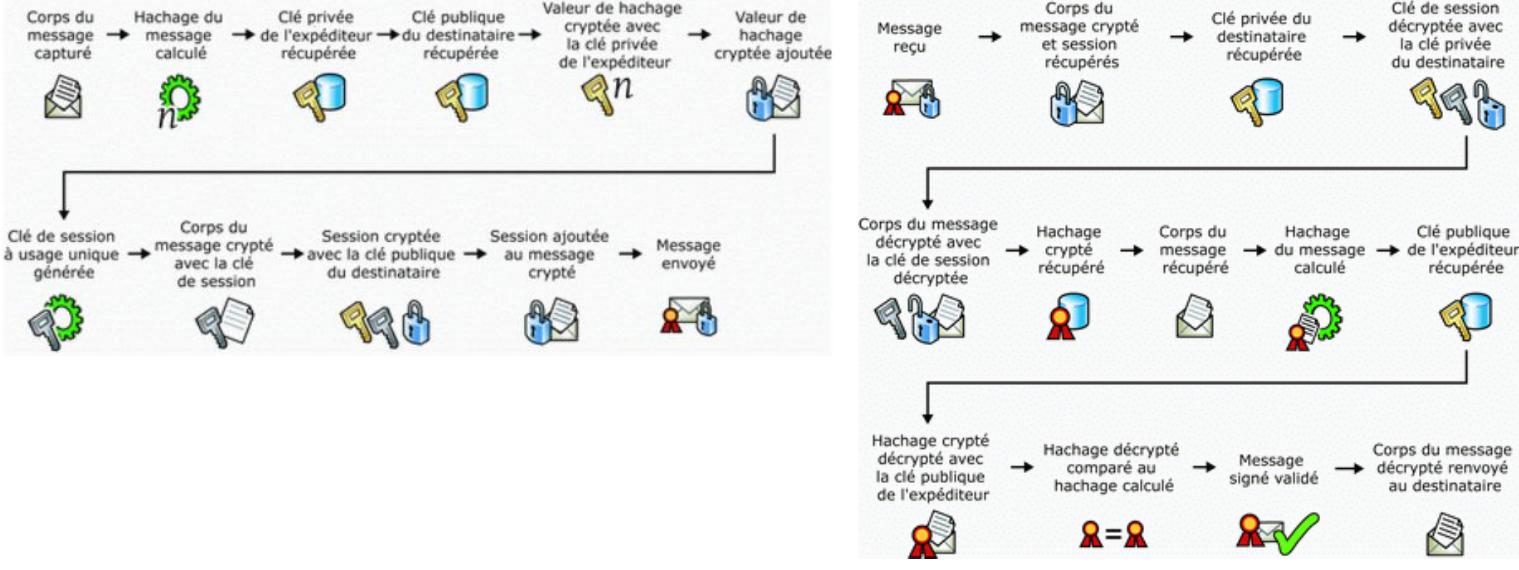
\includegraphics[width=17cm]{images/pack.PNG}
    \caption{Clé de session + signature}
\end{figure}

\section{Avantages/Inconvénient}
\begin{itemize}[label=\textbullet, font=\Large]
    \item Symétrique
    \begin{itemize}[label=\ding{228}, font=\scriptsize]
        \item Avantages
        \begin{itemize}
            \item + facile
            \item + rapide
            \item - de puissance nécessité
            \item Empêche les attaques généralisées étant donné que les clés secrètes sont différentes pour chaque communications
            \item Pas de lien entre les données et la clé
            \item Sans clé, pas moyen de décrypter
        \end{itemize}
        \item Inconvénients
        \begin{itemize}
            \item Manque de sécurité à l'échange des clés
            \item Difficile de gérer et de sécuriser un grand nombre de clés partagées
            \item Ne fournit aucune assurance de l'origine et de l'authenticité d'un message
            \item La même clé est utilisé par les 2
            \item Vulnérables aux attaques par dictionnaire et par force brute
        \end{itemize}
    \end{itemize}
    \item Asymétrique
    \begin{itemize}[label=\ding{228}, font=\scriptsize]
        \item Avantages
        \begin{itemize}
            \item Pratique pour la distribution de clé symétrique
            \item Sécurité renforcée car pas besoin de partager les clés privées
            \item Fourni des signatures numériques
        \end{itemize}
        \item Inconvénients
        \begin{itemize}
            \item Lent
            \item + grande puissance de calcul
            \item Si la clé privée est volée, l'intégralité des messages peuvent être déchiffré
            \item Les messages reçus sont perdu si la clé privée est perdue
            \item Vulnérable au MITM
        \end{itemize}
    \end{itemize}
\end{itemize}

\section{Man in the middle}
Je connais très bien donc pas de synthèse

\section{Infrastructure à clés publiques}
\begin{itemize}[label=\textbullet, font=\Large]
    \item Objectifs
    \begin{itemize}[label=\ding{228}, font=\scriptsize]
        \item Nécessaire pour mettre en place le chiffrement asymétrique
        \item Permet de résourdre le problème d'association entre une entité et une clé publiqué
        \item Désigné par IGC ou PKI (Infrastructure de Gestion de clés ou Public Key Infrastructure)
        \item Fonctions des PKI :
        \begin{itemize}
            \item la génération de couple unique de clés (privée et publique)
            \item la création et la gestion de certificats numériques
            \item la diffusion des clés publiques aux ressources qui la solliciteraient
            \item la certification des clés publiques
        \end{itemize}
    \end{itemize}
    \item Certificats Electroniques
    \begin{itemize}[label=\ding{228}, font=\scriptsize]
        \item Attestent de l'identité numérique des détenteurs de clés publiques
        \item 4 objectifs (ceux de la sécu)
        \begin{itemize}
            \item confidentialité
            \item authenticité
            \item intégrité
            \item non-répudiation
        \end{itemize}
        \item Le certificat est signé avec la clé privé de l'organisme de certification (chiffrement de l’empreinte du certificat avec la clé privée de l’organisme de certification)
        \item Pour valider le certificat :
        \begin{enumerate}
            \item Obtenir la clé publique de l'organisme de certification
            \item Déchiffrer la signature à l'aide de cette clé
            \item Calculer l'empreinte du certificat
            \item Comparer l'empreinte calculée et celle reçue (se trouve à la fin de la signature)
            \item Vérifier que la période de validité du certificat est correcte
        \end{enumerate}
        \item Déjoue le MITM
        \item Certificats auto-signé
        \begin{itemize}
            \item Certificats signé avec la clé privée de l'expéditeur et non celle de l'Infrastructure
        \end{itemize}
    \end{itemize}
    \item Principaux types de certificats :
    \begin{itemize}[label=\ding{228}, font=\scriptsize]
        \item Certificats de messagerie
        \item Authentication IPSec pour un accès distant par VPN
        \item Authentication Internet pour l'HTTPS
        \item Chiffrement des données avec EFS
        \item Signature logiciel
    \end{itemize}
    \item Composant d'une PKI
    \begin{itemize}[label=\ding{228}, font=\scriptsize]
        \item CA (Certificate Authority) : émet et révoque des certificats
        \item RA (Registration Authority) : vérifie l'identité pour le CA
        \item VA (Validation Authority) : détient les certificat accompagné de leur clé publique
        \item End user : Demande, utilise et gère des certificat
        \item Digital Certificates : identifie une personne lors de transactions en ligne
    \end{itemize}
    \item Résumé :
    \begin{enumerate}
        \item Utilisateur demande a RA un certificat
        \item RA vérifie son identité et demande à CA de lui donner le certificat de clé publique
        \item CA donne donne le certificat avec la clé publique de l'utilisateur a Utilisateur
        \item Utilisateur envoie les informations à VA
        \item Quand Utilisateur effectue une action, il signe le mesage avec le certificat de clé publique
        \item Utilisateur envoie son certificat pour prouver son identité au destinataire
        \item Le destinataire vérifie que le certificat est valide
        \item Le VA compare le certificat de clé publique de l'utilisateur avec celui qu’il détient et détermine le résultat (qu'il soit valide ou non).
    \end{enumerate}
\end{itemize}

\section{Algorithmes de cryptographie}
\subsection{Chiffrement par flot et par bloc}
\begin{itemize}[label=\textbullet, font=\Large]
    \item 2 types de chiffrement symetrique
    \begin{itemize}[label=\ding{228}, font=\scriptsize]
        \item Continu (par flot) : agit sur un bit à la fois du message en clair
        \item Par bloc : opère sur le message en clair par groupe de bits (des blocs)
    \end{itemize}
    \item Chiffrement par flot
    \begin{itemize}[label=\ding{228}, font=\scriptsize]
        \item Pas besoin de lire ni de connaître la longueur du message pour le chiffrer
        \item Tente d'imiter le chiffre de Vernam
        \item Généralement combiné par opération XOR avec flux de bits pseudo-aléatoire
        \item Une clé de chiffrement ne doit jamais être utilisée plus de 2 fois
        \item Technique pour ne pas échanger de nouvelles clés en continu :
        \begin{itemize}
            \item Synchronisation d'algorithme via horloge
            \item Vecteur d'initialisation renouvelé et échangé en clair (à ajouter à la clé)
        \end{itemize}
        \item Utilité :
        \begin{itemize}
            \item Téléphonie mobile
            \item Bluetooth
        \end{itemize}
        \item Très bonne performances
        \item Problèmes de sécurité
        \item Exemples :
        \begin{itemize}
            \item RC-4 (mal utilisé par le WEP du WiFi)
            \item A5/1 (Utilisé dans la téléphonie mobile GSM)
        \end{itemize}
    \end{itemize}
    \item Chiffrement par bloc :
    \begin{itemize}[label=\ding{228}, font=\scriptsize]
        \item Le message est découpé en blocs de $n$ blocs de bit, tous de même taille, ensuite chaque blocs est chiffré
        \begin{itemize}
            \item Si la longueur du message n'est pas un multiple de la longueur du bloc, on utilise le padding (bourrage) pour compléter le dernier bloc
        \end{itemize}
        \item Existe plusieurs technique de chiffrement par bloc :
        \begin{itemize}
            \item EBC (Electronic CodeBook) : 
            \begin{itemize}
                \item Chaque bloc est chiffré séparémment les uns après les autres
                \item Non recommendé car si même contenu alors même chiffrement
                \item On obtient un dictionnaire de codes avec les correspondances entre le clair et le chiffré
                \begin{figure}[H]
                    \centering
                    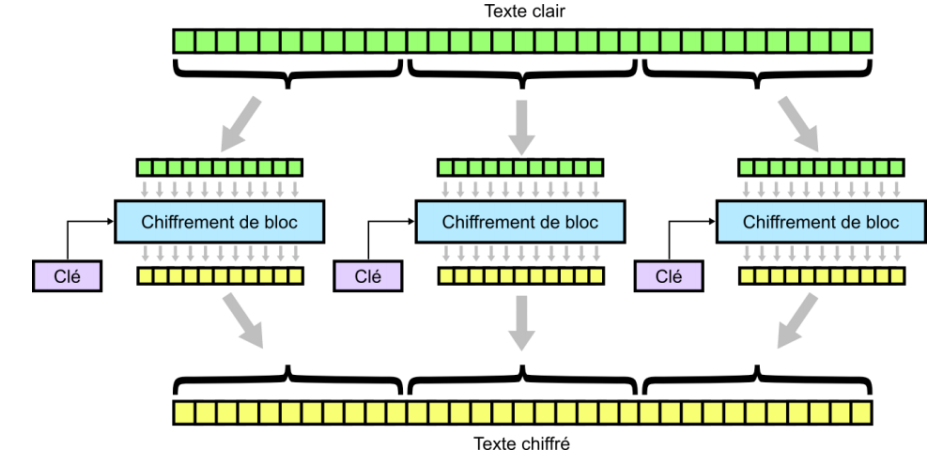
\includegraphics[width=18cm]{images/EBC.PNG}
                    \caption{EBC}
                \end{figure}
            \end{itemize}
            \item CBC (Cipher Block Chaining)
            \begin{itemize}
                \item "OU exclusif" sur chaque block avec le chiffrement du bloc précent
                \item Pour rendre chaque message unique, un vecteur d'initialisation (IV) est utilisé
                \begin{figure}[H]
                    \centering
                    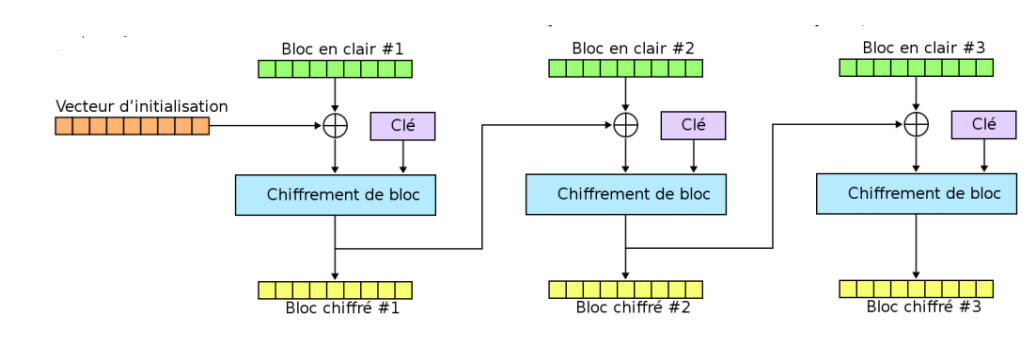
\includegraphics[width=15cm]{images/CBC.PNG}
                    \caption{CBC}
                \end{figure}
            \end{itemize}
            \item CFB (Cipher FeedBack) et OFB (Output FeedBack)
            \begin{itemize}
                \item Utilisé comme un générateur pseudo-aléatoire de clés en essayant de simuler un chiffrement par masque jetable
                \item Exemple : DES, AES
                \begin{figure}[H]
                    \centering
                    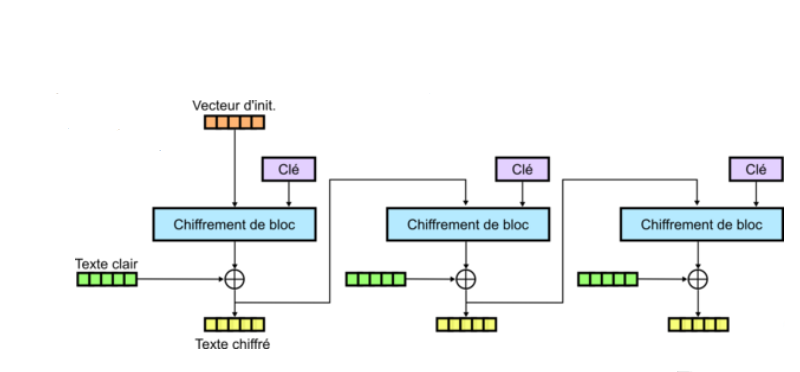
\includegraphics[width=15cm]{images/CFB.PNG}
                    \caption{CFB et OFB}
                \end{figure}
            \end{itemize}
        \end{itemize}
    \end{itemize}
\end{itemize}

\subsection{DES}
\begin{itemize}[label=\textbullet, font=\Large]
    \item Description de la clé
    \begin{itemize}[label=\ding{228}, font=\scriptsize]
        \item Clé = chaîne de 64 bits
        \item Seuls 56 bits servent réellement à définir la clé
        \item Les bits 8,16,24,32,40,48,56,64 = bits de parité
        \item $2^{56}$ clés possibles = 72 millions de milliard de possibilités
    \end{itemize}
    \item DES cassé en 3 semaines en 1997
    \item Fonctionnement :
    \begin{itemize}[label=\ding{228}, font=\scriptsize]
        \item 16 sous clés sont créées à partir de la clé de 56 bits
        \item Utilise des combinaisons, substitutions, permutations (entre texte et clé)
        \item Chaque bloc de 64 bits du texte est calculé une permutation et on divise les 64 bits en 32
        \item On applique 16 tours, chacun à l'aide d'une sous-clé et d'un même schéma de substitutions et de permutations
        \item On regroupe les 2 blocs de 32 bits et on permute
        \item Le déchiffrement ce fait dans l'ordre inverse 
        \begin{figure}[H]
            \centering
            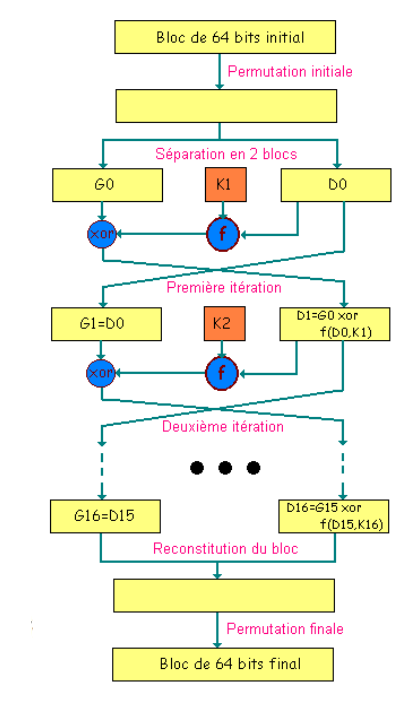
\includegraphics[width=5cm]{images/DES.PNG}
            \caption{DES}
        \end{figure}
    \end{itemize}
\end{itemize}

\subsection{3DES}
\begin{itemize}[label=\textbullet, font=\Large]
    \item Etant donné que DES ne pouvais plus être utilisé, 3DES est créé en solution provisoire
    \item Fonctionnement :
    \begin{itemize}[label=\ding{228}, font=\scriptsize]
        \item 2 clés de 56 bits
        \item 3 chiffrement DES en chaîne
        \item Augmente significativement la sécurité de DES (demande plus de ressources)
    \end{itemize}
    \item Variante :
    \begin{figure}[H]
        \centering
        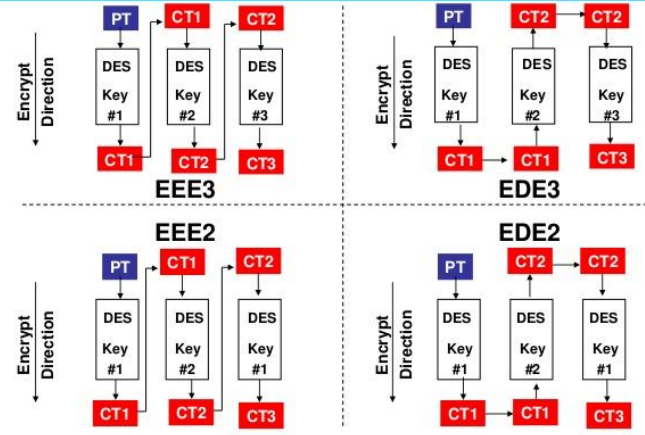
\includegraphics[width=9cm]{images/variante.PNG}
        \caption{Variante de 3DES - DES-E...}
    \end{figure}
\end{itemize}

\subsection{AES - Advanced Encryption Standard}
\begin{itemize}[label=\textbullet, font=\Large]
    \item Belge
    \item Fonctionnement
    \begin{itemize}[label=\ding{228}, font=\scriptsize]
        \item Chiffrement par bloc
        \item clés de : 128, 192, 256
        \item Blocs de 128 bits
        \item Les blocs sont encodés en plusieurs cycles consécutifs
        \item A chaque cycle : permutation, substitution, XOR, ...
    \end{itemize}
    \item Utilité
    \begin{itemize}[label=\ding{228}, font=\scriptsize]
        \item WPA2
        \item SSH
        \item IPSec
        \item Chiffrement des archives compressés
    \end{itemize}
\end{itemize}

\subsection{RC}
\begin{itemize}[label=\textbullet, font=\Large]
    \item Inventé par l'inventeur du MD5
    \item Employé en raison de leur vitesse et parce que la longeur de la clé est variable
    \item RC2
    \begin{itemize}[label=\ding{228}, font=\scriptsize]
        \item Conçu pour remplacer le DES
        \item Chiffrement par bloc de taille de clé variable
    \end{itemize}
    \item RC4
    \begin{itemize}[label=\ding{228}, font=\scriptsize]
        \item Chiffrement par flux le plus utilisé au monde
        \item Utilisé pour le chiffrement de fichiers et pour les communications sécurisées (ex : SSL)
        \item Considéré comme sécurisé bien qu'il puisse être implémenté de manière non sécurisé (WEP)
    \end{itemize}
\end{itemize}

\subsection{Diffie-Hellman}
\begin{itemize}[label=\textbullet, font=\Large]
    \item Utilisé pour échanger des clés en toute sécurité
    \item Utiilité :
    \begin{itemize}[label=\ding{228}, font=\scriptsize]
        \item Algorithme mathématique qui permet de générer un secret partagé sur 2 systèmes sans avoir à le communiquer
        \item Pas vraiment de clé symétrique échangée entre l'expéditeur et le destinataire
        \item VPN IPsec, SSL TLS, quand des données SSH sont échangées
    \end{itemize}
    \item Analogie :
    \begin{figure}[H]
        \centering
        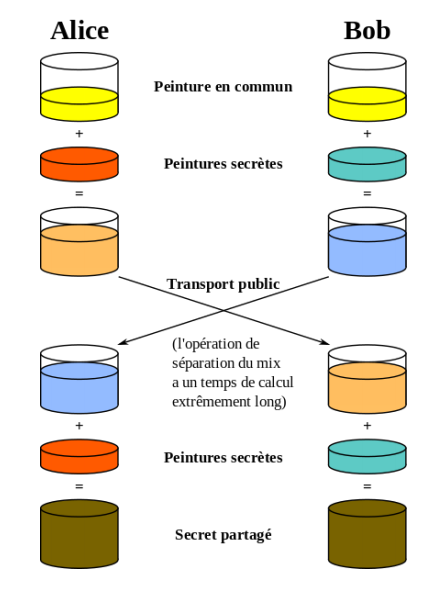
\includegraphics[width=7cm]{images/DH.PNG}
        \caption{Analogie Diffie-Hellman}
    \end{figure}
    \item Fonctionnement :
    \begin{itemize}[label=\ding{228}, font=\scriptsize]
        \item Utilise les modulos
        \item 38 modulo 7
        \item 1ère étape :
        \begin{itemize}
            \item Alice et Bob choisissent ensemble 2 nombres (p: un nombre premier, g : tel quel 1<g<p (generator))
            \item Nombre public
        \end{itemize}
        \item 2ème étape :
        \begin{itemize}
            \item Alice génère aléatoirement un grand nombre A
            \item pareil pour Bob avec un nombre B
            \item A et B restent secret
        \end{itemize}
        \item 3ème étape :
        \begin{itemize}
            \item Alice calcule $P_A = g^A$ $mod$ $p$ et transmet le résultat à Bob
            \item Bob calcule $P_B = g^B$ $mod$ $p$ et transmet le résultat à Alice
        \end{itemize}
        \item 4ème étape :
        \begin{itemize}
            \item La clé secrète symétrique est $k = g^{AB}$ $mod$ $p$
            \item Alice peut calculer k à partir de $A$ et $P_B (g^B$ $mod$ $p)$
            \item Bob peut calculer k à partir de $B$ et $P_A (g^A$ $mod$ $p)$
            \begin{figure}[H]
                \centering
                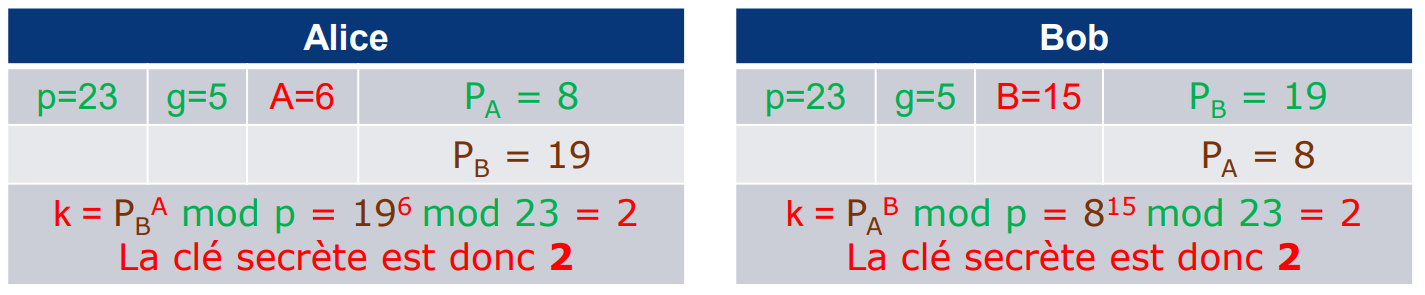
\includegraphics[width=15cm]{images/exempledh.PNG}
                \caption{Exemple Diffie-Hellman}
            \end{figure}
        \end{itemize}
    \end{itemize}
    \item Secret
    \begin{itemize}[label=\ding{228}, font=\scriptsize]
        \item Si Eve écoute la conversation, elle ne pourra pas trouver $k$
        \item Nombres utilisés sont en réalité d'environ 1024 bits (309 chiffres) donc complexe
    \end{itemize}
    \item Utilisation
    \begin{itemize}[label=\ding{228}, font=\scriptsize]
        \item Exige la simultanéité des actions d'Alice et de Bob
        \item Protocol surplanté par des méthodes de type RSA pour lesquels on met à disposition une clé publique
        \item Utilisé pour l'appariement d'objets Bluetooth
    \end{itemize}
\end{itemize}

\subsection{RSA}
\begin{itemize}[label=\textbullet, font=\Large]
    \item Très démocratisé et présent presque partout
    \item Système à clé publique
    \item Fonctionnement :
    \begin{itemize}[label=\ding{228}, font=\scriptsize]
        \item P et Q étant 2 nombres premiers aléatoire
        \item $N = P.Q$ = Modulus
        \item $\phi = (P-1)(Q-1)$
        \item $E$ aléatoire tel que $1 < E < \phi$ et que $E$ et $\phi$ soient premier entre-eux ($E$ n'est pas forcément premier mais doit être impair)
        \item $D$ calculé tel que $(D.E - 1)$ divisible par $\phi$
        \begin{itemize}

            \item Il faut trouver un entier $X$ tel que D soit entier et que :
            \item $D = \frac{(X.\phi) + 1}{E}$
        \end{itemize}
        \item $E$ = exposant public ( (N, E) = clé publique)
        \item $D$ = exposant privé  ( (N, D) = clé privée)
        \item Taille de P \& Q > 1000 bits (détruit après génération des clés)
        \item Chiffrement :
        \begin{itemize}
            \item $C = T^E$ $mod$ $N$
            \item T = texte clair
            \item C = texte chiffré
        \end{itemize}
        \item Déchiffrement :
        \begin{itemize}
            \item $T = C^D$ $mod$ $N$
        \end{itemize}
    \end{itemize}
    \item Exemples avec petites valeurs:
    \begin{itemize}[label=\ding{228}, font=\scriptsize]
        \item P = 11
        \item Q = 3
        \item N = 33 (P.Q)
        \item $\phi = (P-1).(Q-1) = 20$
        \item E par exemple = 3 (3 < 20, 3 est premier et ne divise pas 20, E et $\phi$ sont premier entre eux)
        \item D calulé :
        \begin{itemize}
            \item $D.3 - 1$ doit être divisible par 20
            \item $D = \frac{(X.20 + 1)}{3}$
            \item Avec X = 1 $\rightarrow$ D = 7
        \end{itemize}
        \item Chiffrer 13 : $C = 13^3$ $mod$ $33 = 19$
        \item Pour déchiffrer 19 : $T = 19^7$ $mod$ $33 = 13$
    \end{itemize}
\end{itemize}

\subsection{MD5 et SHA}
\begin{itemize}[label=\textbullet, font=\Large]
    \item MD5
    \begin{itemize}[label=\ding{228}, font=\scriptsize]
        \item Séquence complexe d'opération binaires simples (XOR, rotations)
        \item Empreinte de 128 bits
        \item Déprécié
    \end{itemize}
    \item SHA
    \begin{itemize}[label=\ding{228}, font=\scriptsize]
        \item Similaire à MD5
        \item 3 générations : sha-1, sha-2 et sha-3
    \end{itemize}
    \item Sécurité :
    \begin{itemize}[label=\ding{228}, font=\scriptsize]
        \item Failles de sécurité dans SHA-1 et MD5
        \item Il faut utiliser SHA-256 ou version ultérieure
    \end{itemize}
\end{itemize}

\subsection{SSL et TLS}
\begin{itemize}[label=\textbullet, font=\Large]
    \item Chiffrement asymétrique pour un échange de clé symétrique + certificats
    \item Fonctionnement :
    \begin{enumerate}
        \item Le navigateur envoie une requête pour se connecter grâce au SSL ou TLS
        \item Le serveur envoie ses certificats qui contiennent sa clé publique
        \item Le client vérifie le certificat et si il est bon, il chiffre une clé de session avec la clé publique du serveur et lui envoie
        \item Le serveur déchiffre la clé de session avec sa clé privée
        \item Ils communiquent ensuite grâce au chiffrement de cette clé de session
    \end{enumerate}
\end{itemize}















\end{document}